\section{Analiza i~wizualizacja danych} \label{sec:analysis}
Uruchomienie wszystkich scenariuszy symulacji spowodowało wygenerowanie dużej ilości danych ($\sim$300GB) rozłożonej na tysiące plików. W~celu analizy takiej ilości danych napisany został skrypt w~języku Ruby \cite{ruby}, którego zadaniem była decymacja oraz fuzja wszystkich plików.

Do analizy oraz wizualizacji danych wykorzystany został język R wraz z~pakietem ggplot2. Dla ułatwienia porównań wykresy zostały zebrane w~większe macierze i~przedstawione w~załączniku. Dla każdej topologii sieci powstały dwie takie macierze: jedna zawierająca wykresy liczby aktywnych czujników, druga natomiast zawiera wykresy przedstawiające sumę energii w~całej sieci. Na wykresach energii sieci za pomocą przerywanych pionowych linii oznaczony został czas, po którym nastąpiło wyłączenie pierwszego węzła w~sieci z~powodu zbyt niskiego poziomu energii (poniżej 10\%). Od tego momentu uważa się, że sieć działa w~trybie niestabilnym.
Każdy protokół został przetestowany z~następującymi parametrami wejściowymi:
\begin{itemize}
	\item Rozmiar pakietu danych: 5B, 50B, 500B, 5000B
	\item Czas po którym następuje wygenerowanie nowego pakietu danych: 5s, 10s, 15s, 20s
	\item Liczba węzłów sieci: 20, 200
\end{itemize}

Dodatkowo, po przeprowadzeniu wszystkich scenariuszy testowych oraz analizie wyników okazało się, że protokół SPIN oraz Flood uzyskały bardzo zbliżone rezultaty, a~co za tym idzie ich wykresy pokrywają się w~każdym przypadku. Wszelkiego rodzaju spostrzeżenia i~obserwacje (zawarte w~opisach wykresów) dotyczące protokołu SPIN będą się odnosić również do protokołu Flood. 
W przypadku tych protokołów dezaktywacja węzłów sieci przebiega gwałtownie oraz lawinowo - większość węzłów sieci zostaje wyłączonych w~zbliżonym czasie.

\newpage
Na wykresach została przedstawiona zależność pomiędzy liczbą aktywnych węzłów w~zależności od odstępów pomiędzy kolejnymi pakietami.Sieć składała się z~dwudziestu węzłów, które rozmieszczone zostały zgodnie z~rozkładem normalnym.

Dla pakietów o~rozmiarze 5B można zauważyć najdłuższy czas działania sieci do zakończenia pracy ostatniego węzła. Dla tego pakietu najdłużej działającymi protokołami były ALEACH i~LEACH DCHS. Zależność ta była najbardziej widoczna w~przypadku odstępów równych 20s. Na uwagę zasługuje również wzrost czasu działania sieci wraz ze wzrostem okresu generowania pakietów z~danymi.

\begin{figure}[H]
	\begin{center}
		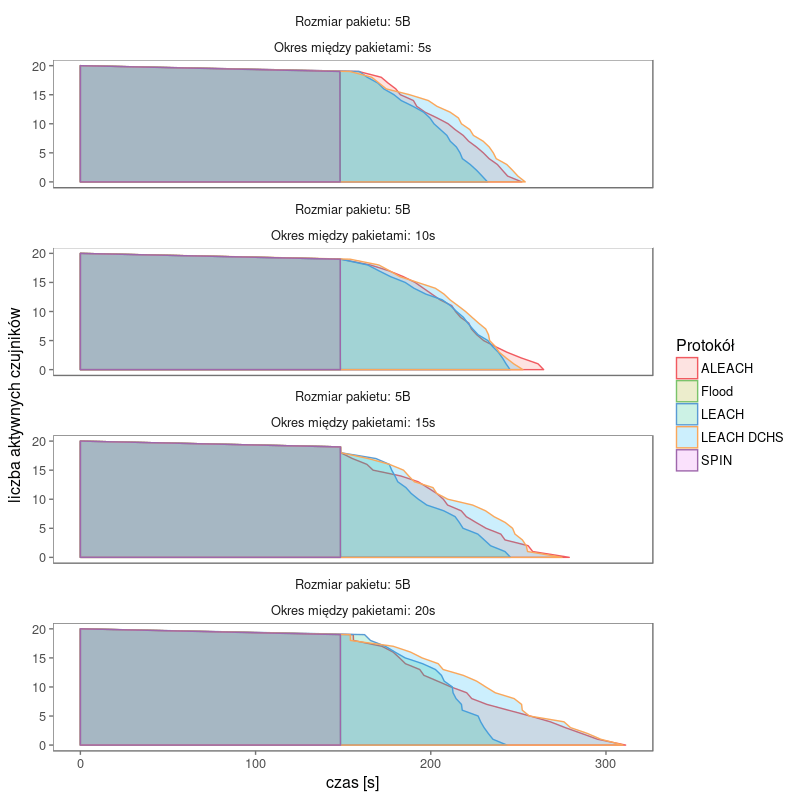
\includegraphics[scale=0.6]{\ImgPath/charts/alive_nodes_normal_20sensors_row1.png}
	\end{center}
	\caption{Aktywne węzły - liczba czujników: 20, rozmiar pakietu danych: 5B, rozkład normalny}
\end{figure}

Wykresy pakietów 50B i~500B wydają się relatywnie podobne, jednak można zauważyć różnice pomiędzy nimi. Główną różnicą jest dłuższy czas działania sieci w~przypadku pakietów 50B. Wykresy te prezentują znaczne podobieństwa w~przebiegu protokołów, wyjątkiem jest protokół ALEACH. W~wykresach dla pakietów 50B z~odstępami równymi 10s i~20s działał on zdecydowanie najdłużej. W~przypadku wykresu z~odstępami 20s działanie było dłuższe o~ponad 50 sekund. Tak dobrych wyników protokół ten nie osiągał już w~przypadku pakietu 500B. W~tym przypadku widać podobieństwo w~długości działania sieci. Rozbieżności są widoczne jedynie na wykresie o~odstępach 20s, gdzie najdłużej działającym protokołem był LEACH DCHS. 

\begin{figure}[H]
	\begin{center}
		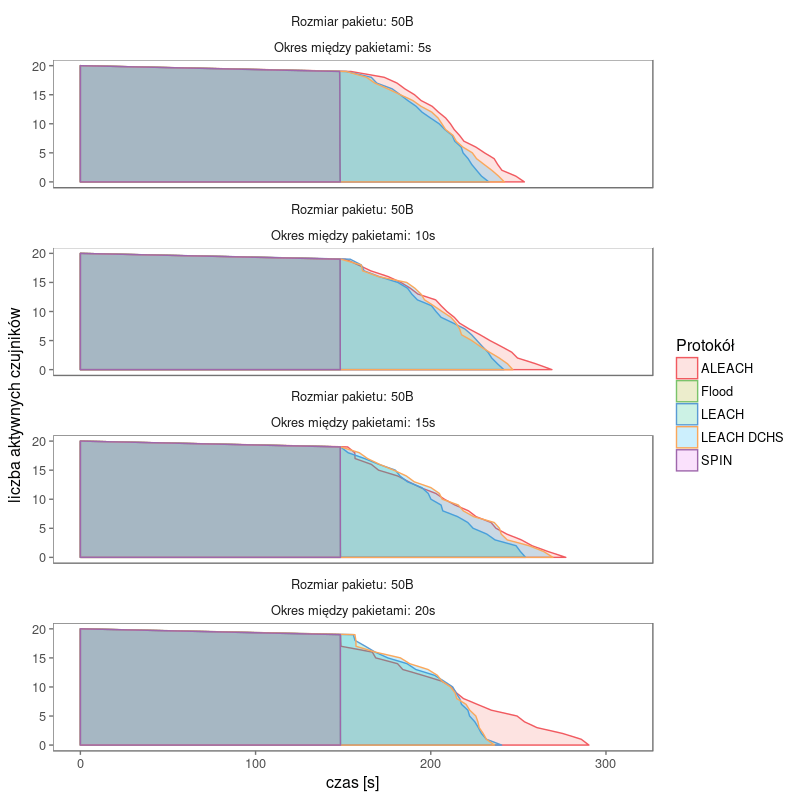
\includegraphics[scale=0.6]{\ImgPath/charts/alive_nodes_normal_20sensors_row2.png}
	\end{center}
	\caption{Aktywne węzły - liczba czujników: 20, rozmiar pakietu danych: 50B, rozkład normalny}
\end{figure}

\begin{figure}[H]
	\begin{center}
		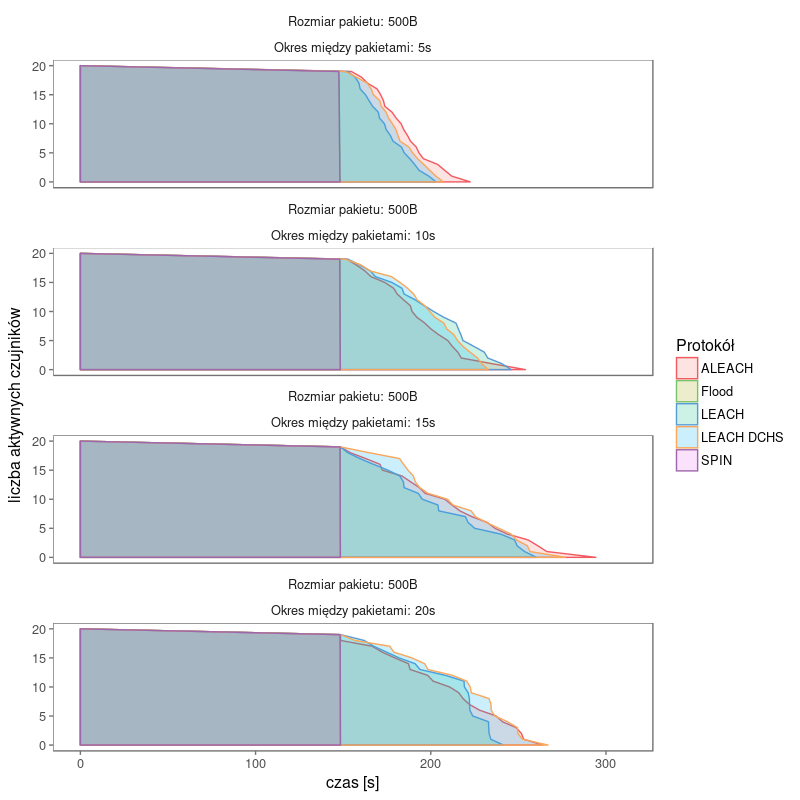
\includegraphics[scale=0.6]{\ImgPath/charts/alive_nodes_normal_20sensors_row3.png}
	\end{center}
	\caption{Aktywne węzły - liczba czujników: 20, rozmiar pakietu danych: 500B, rozkład normalny}
\end{figure}

Dla pakietów o~rozmiarze 5000B można zauważyć najkrótszy czas działania wszystkich pakietów. Dla tych, w~których przerwa wynosiła 5s, 10s i~15s ostatni węzeł kończył pracę już przed 200 sekundą. Warto nadmienić, że dla pakietów z~przerwami 5s i~20s protokołem działającym najdłużej był ALEACH. 

\begin{figure}[H]
	\begin{center}
		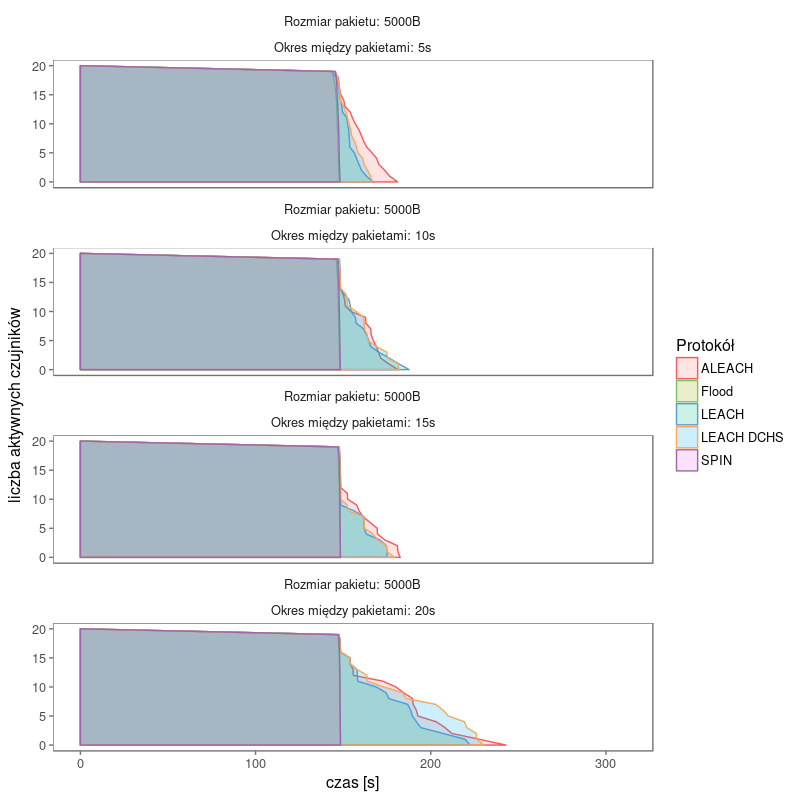
\includegraphics[scale=0.6]{\ImgPath/charts/alive_nodes_normal_20sensors_row4.png}
	\end{center}
	\caption{Aktywne węzły - liczba czujników: 20, rozmiar pakietu danych: 5000B, rozkład normalny}
\end{figure}
 

Na wykresach przedstawiono zależność pomiędzy sumą energii sieci w~zależności od czasu, rozmiaru  i~rodzaju pakietu. Sieć składała się z~20 węzłów początkowych rozmieszczonych zgodnie z~rozkładem normalnym.
  
Ogólną tendencją, którą można zauważyć na wykresach jest najwolniejszy spadek energii zgromadzonej w~sieci dla pakietów wysyłanych w~odstępach 20s. Sieć najszybciej traci energię dla protokołów SPIN oraz Flood. Protokołem, który najwolniej wytracał energię, jest ALEACH, jednak ta tendencja nie została zaobserwowana we wszystkich eksperymentach.

Dla pakietów równych 5B można zaobserwować najdłuższy wykres, najwolniejszy spadek energii sieci. Wykres ten był przypisany do pakietów danych wysyłanych z~odstępami o~wartości 20s. W~tym przypadku najdłużej działającymi protokołami były ALEACH i~LEACH DCHS. Na wykresach dla pakietów danych o~rozmiarze 5B można zaobserwować relatywnie dużą różnicę pomiędzy SPIN a~pozostałymi protokołami. Ten pierwszy zdecydowanie szybciej zużywa energię zgromadzoną w~sieci.

\begin{figure}[H]
	\begin{center}
		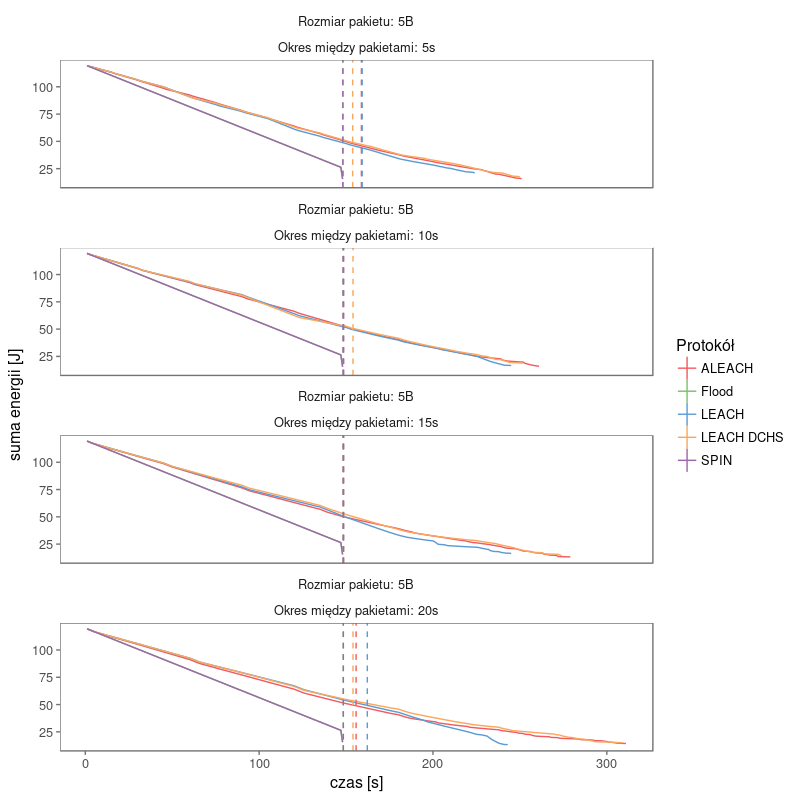
\includegraphics[scale=0.6]{\ImgPath/charts/stored_energy_normal_20sensors_row1.png}
	\end{center}
	\caption{Energia sieci - liczba czujników: 20, rozmiar pakietu danych: 5B, rozkład normalny}
\end{figure}

Wykresy pakietów o~rozmiarach 50B i~500B wydają się podobne. Różnicą, którą można zaobserwować jest zmniejszenie się rozbieżności pomiędzy SPIN, a~pozostałymi protokołami. Najwyraźniej zmianę tą obserwuje się w~pakietach wysyłanych co 5s dla rozmiarów 50B i~500B. Tendencją w~wykresach pakietów o~rozmiarze 500B jest zwiększanie się różnicy między SPIN, a~pozostałymi protokołami wraz ze wzrostem odstępu między wysyłką kolejnych pakietów danych. Na uwagę zasługuje również wykres dla pakietów o~rozmiarze 50B wysyłanych w~odstępie 20s. Zauważono, że sieć używająca protokołu ALEACH wyraźnie dłużej wytraca energię niż w~przypadku pozostałych protokołów. 

\begin{figure}[H]
	\begin{center}
		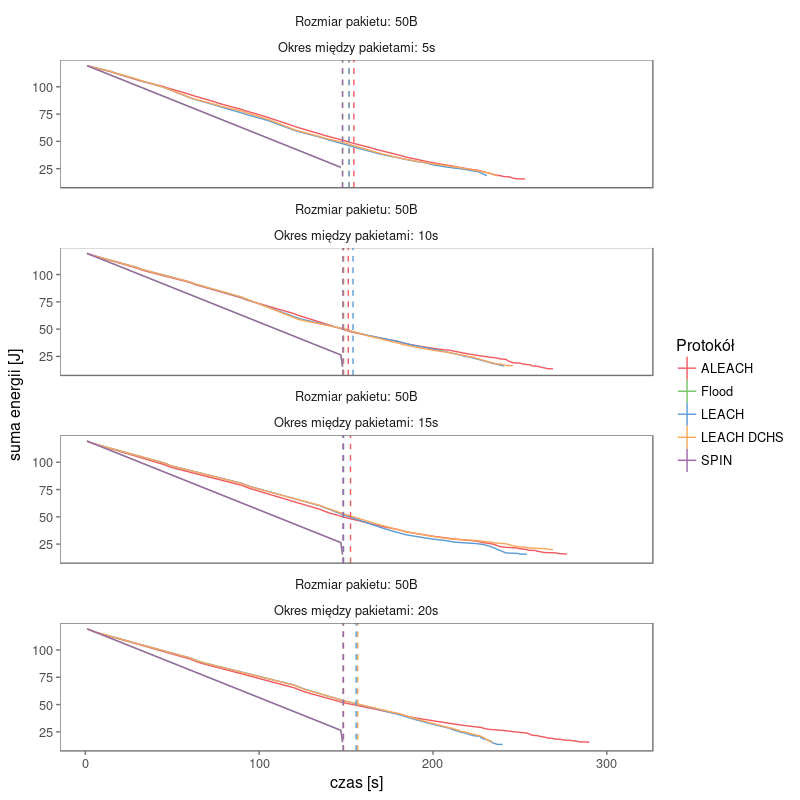
\includegraphics[scale=0.6]{\ImgPath/charts/stored_energy_normal_20sensors_row2.png}
	\end{center}
	\caption{Energia sieci - liczba czujników: 20, rozmiar pakietu danych: 50B, rozkład normalny}
\end{figure}

\begin{figure}[H]
	\begin{center}
		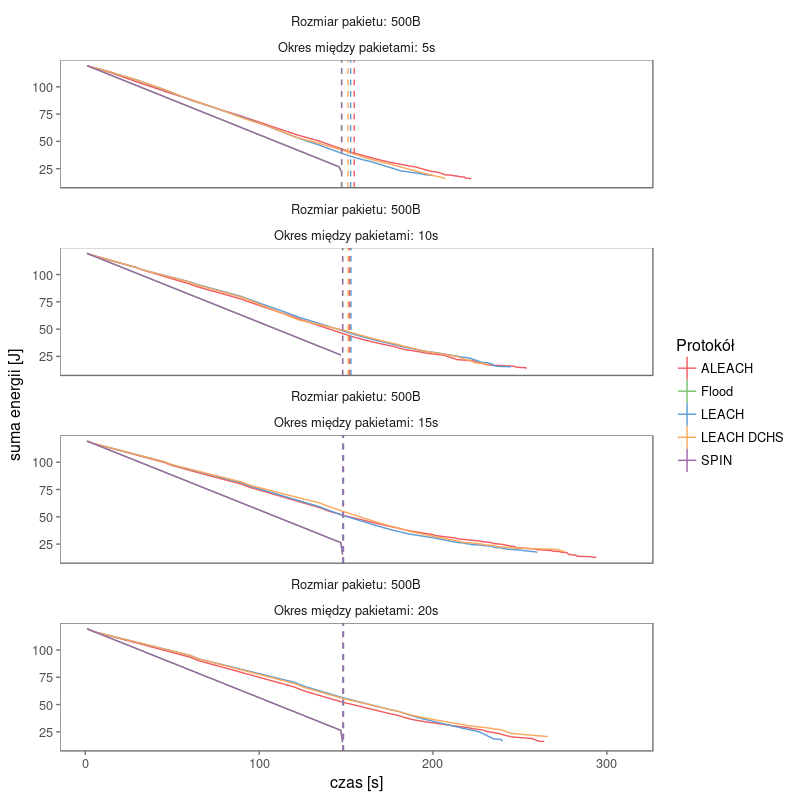
\includegraphics[scale=0.6]{\ImgPath/charts/stored_energy_normal_20sensors_row3.png}
	\end{center}
	\caption{Energia sieci - liczba czujników: 20, rozmiar pakietu danych: 500B, rozkład normalny}
\end{figure}

Wykresami, które różnią się od pozostałych są te o~rozmiarze pakietu danych wynoszącym 5000B. Nie obserwuje się tu różnicy pomiędzy SPIN, a~pozostałymi protokołami. Wyjątkiem jest wykres dla pakietu z~okresami odstępu 20s, gdzie SPIN nieznacznie szybciej zużywa energię sieci. Zauważono, że ogólna suma energii węzłów dla pakietów o~rozmiarze 5000B jest szybciej wytracana niż w~przypadku pozostałych wykresów.

\begin{figure}[H]
	\begin{center}
		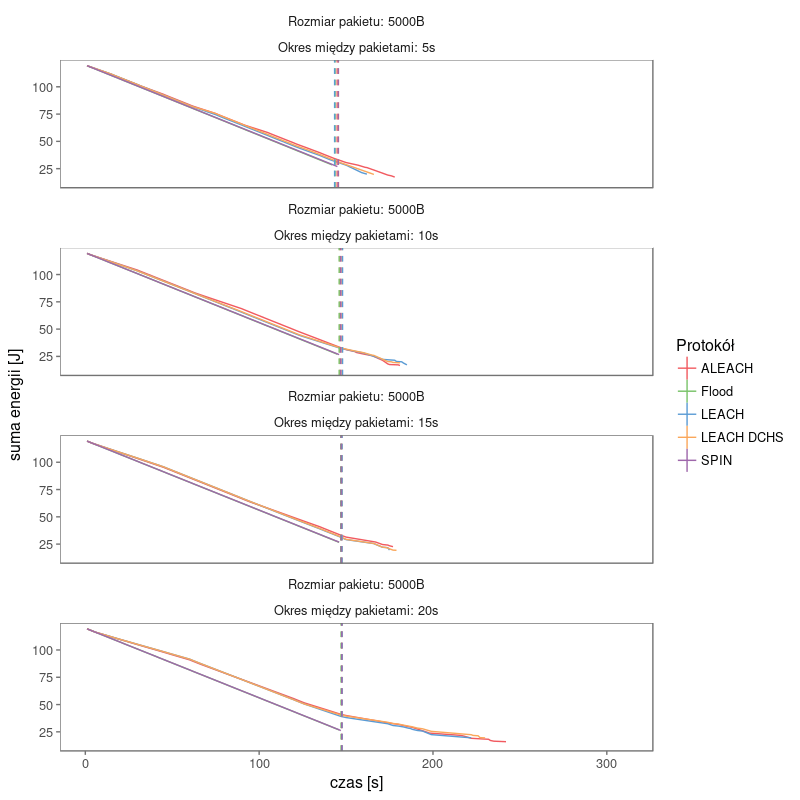
\includegraphics[scale=0.6]{\ImgPath/charts/stored_energy_normal_20sensors_row4.png}
	\end{center}
	\caption{Energia sieci - liczba czujników: 20, rozmiar pakietu danych: 5000B, rozkład normalny}
\end{figure}

Na wykresach przedstawiono liczbę aktywnych czujników w~zależności od rozmiaru pakietu, okresami między pakietami i~rodzajem protokołu. Sieć składała się z~dwustu węzłów, które rozmieszczone zostały zgodnie z~rozkładem normalnym.

Ogólnym trendem, który można zauważyć wśród wykresów jest szybsze zmniejszanie się liczby aktywnych czujników wraz ze wzrostem rozmiaru pakietu. Można zauważyć, że często najdłużej czujniki pozostawały aktywne w~czasie pracy protokołu LEACH DCHS oraz LEACH. Inną istotną zależnością jest wzrost liczby aktywnych czujników skorelowany ze wzrostem okresu między pakietami.
 
Dla rozmiaru pakietu 5B można zaobserwować najwyższe wartości aktywnych czujników, które dodatkowo rosną wraz ze zwiększającym się okresem między pakietami. Na uwagę zasługuje wykres, w~którym pakiety danych wysyłane są co 10s. Tu największa liczba czujników po 300 sekundzie była odnotowana w~przypadku zastosowania protokołu LEACH. Na pozostałych wykresach tej grupy najwyższą liczbę czujników odnotowano dla protokołu LEACH DCHS.

\begin{figure}[H]
	\begin{center}
		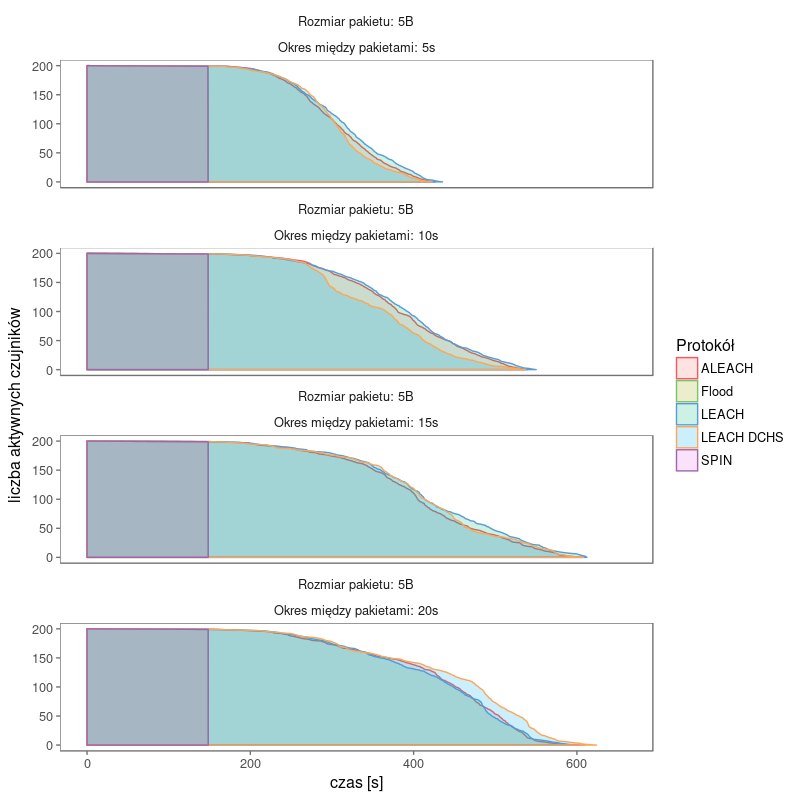
\includegraphics[scale=0.6]{\ImgPath/charts/alive_nodes_normal_200sensors_row1.png}
	\end{center}
	\caption{Aktywne węzły - liczba czujników: 200, rozmiar pakietu danych: 5B, rozkład normalny}
\end{figure}


Podobne zależności odnotowano w~przypadku rozmiaru pakietu 50B. Wyjątkiem jest wykres o~okresach między pakietami równymi 5s. Tu czujniki wykorzystujące protokół LEACH DCHS szybciej ulegały dezaktywacji niż w~przypadku pozostałych protokołów. 

\begin{figure}[H]
	\begin{center}
		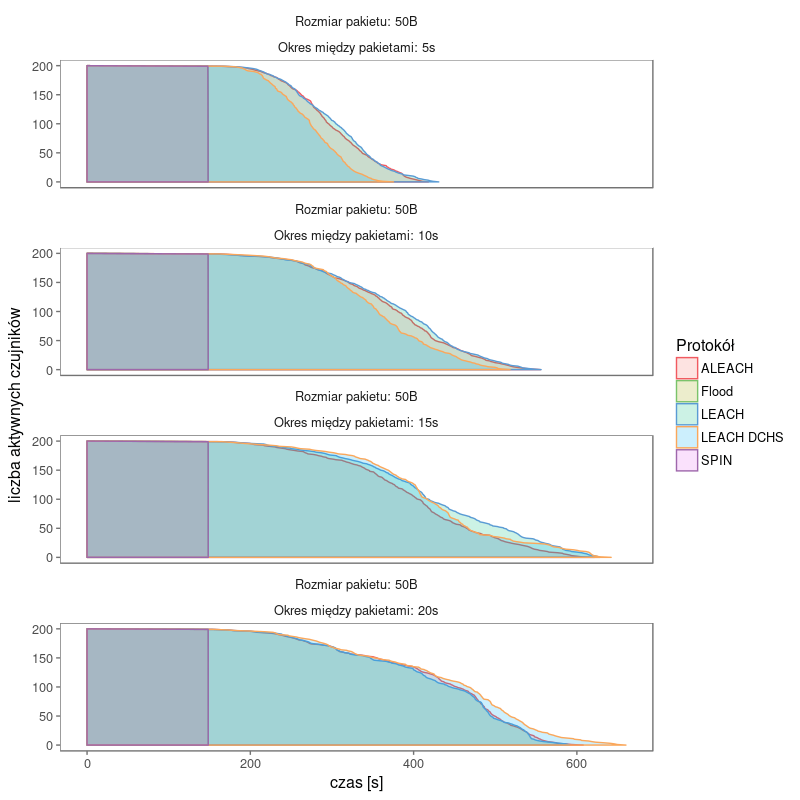
\includegraphics[scale=0.6]{\ImgPath/charts/alive_nodes_normal_200sensors_row2.png}
	\end{center}
	\caption{Aktywne węzły - liczba czujników: 200, rozmiar pakietu danych: 50B, rozkład normalny}
\end{figure}


Można zaobserwować zmianę pewnych tendencji w~przypadku pakietów o~rozmiarze 500B. Tu szybciej zmniejszała się liczba aktywnych czujników, a~sama długość ich działania jest krótsza niż w~przypadku pakietów o~rozmiarze 5B i~50B. Warto zwrócić uwagę na wykres o~okresie między pakietami równym 10s. Tu najdłużej aktywnymi czujnikami były te, w~których zastosowano protokół LEACH i~ALEACH.

\begin{figure}[H]
	\begin{center}
		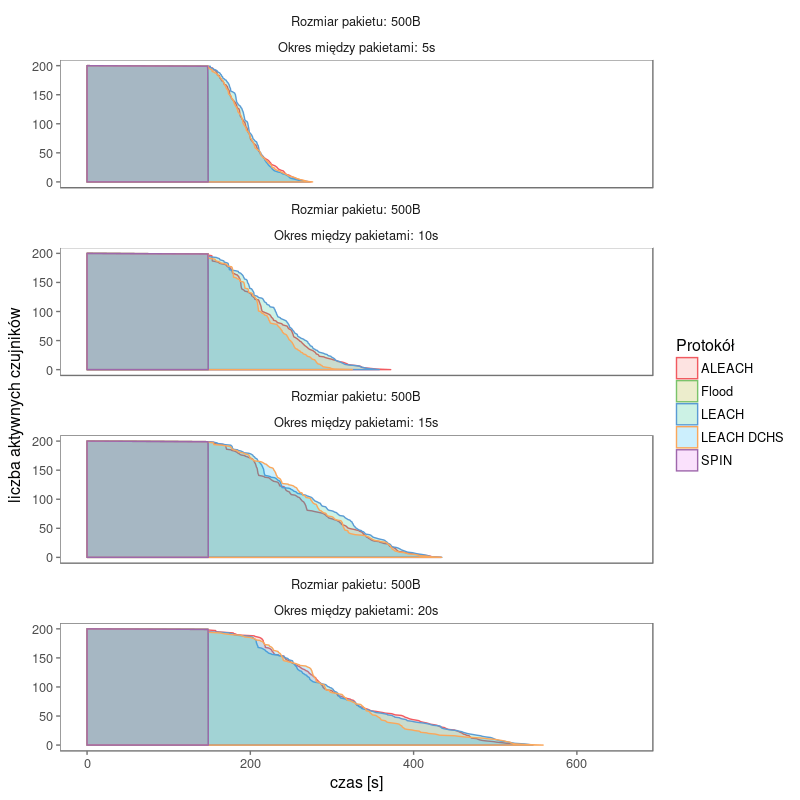
\includegraphics[scale=0.6]{\ImgPath/charts/alive_nodes_normal_200sensors_row3.png}
	\end{center}
	\caption{Aktywne węzły - liczba czujników: 200, rozmiar pakietu danych: 500B, rozkład normalny}
\end{figure}

 
Wykresy protokołów dla rozmiaru 5000B są zdecydowanie najkrótsze. Na uwagę zasługuje ten z~okresami między pakietami równymi 5s, dla którego czas działania sieci nie przekracza 200 sekund. Najdłuższy wykres z~tej grupy, w~którym przerwy były równe 20s, opisuje sieć działającą niecałe 400 sekund, gdzie w~pozostałych protokołach dla tej długości okresów między pakietami czas ustania aktywności ostatniego czujnika przypadał na około 600 sekund od czasu rozpoczęcia. Istotne jest również, to że w~tej grupie najszybciej spadała liczba aktywnych czujników.

\begin{figure}[H]
	\begin{center}
		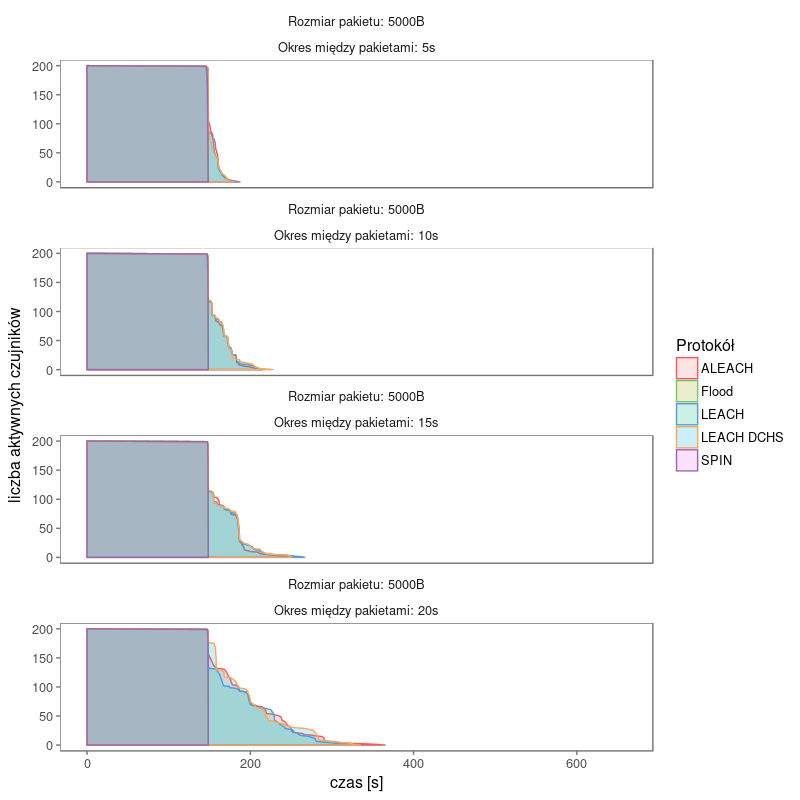
\includegraphics[scale=0.6]{\ImgPath/charts/alive_nodes_normal_200sensors_row4.png}
	\end{center}
	\caption{Aktywne węzły - liczba czujników: 200, rozmiar pakietu danych: 5000B, rozkład normalny}
\end{figure}
 

Na wykresach przedstawiono sumę energii wyrażoną w~dżulach w~zależności od czasu, rozmiaru pakietu, długości okresów między pakietami i~rodzajem protokołu. Sieć składała się z~dwustu węzłów, które rozmieszczone zostały zgodnie z~rozkładem normalnym.

Największą różnicę pomiędzy protokołem SPIN, a~pozostałymi protokołami można zauważyć w~pakietach o~rozmiarze 5B. SPIN dużo szybciej zużywa energię sieci, a~jego wykres kończy się zazwyczaj w~pierwszej połowie długości pozostałych protokołów. Tendencja, która jest zauważalna w~tej grupie to wydłużający się czas zużycia energii wraz ze wzrostem okresów między pakietami. Warto nadmienić, że protokoły ALEACH, LEACH i~LEACH DCHS miały relatywnie podobny przebieg.

\begin{figure}[H]
	\begin{center}
		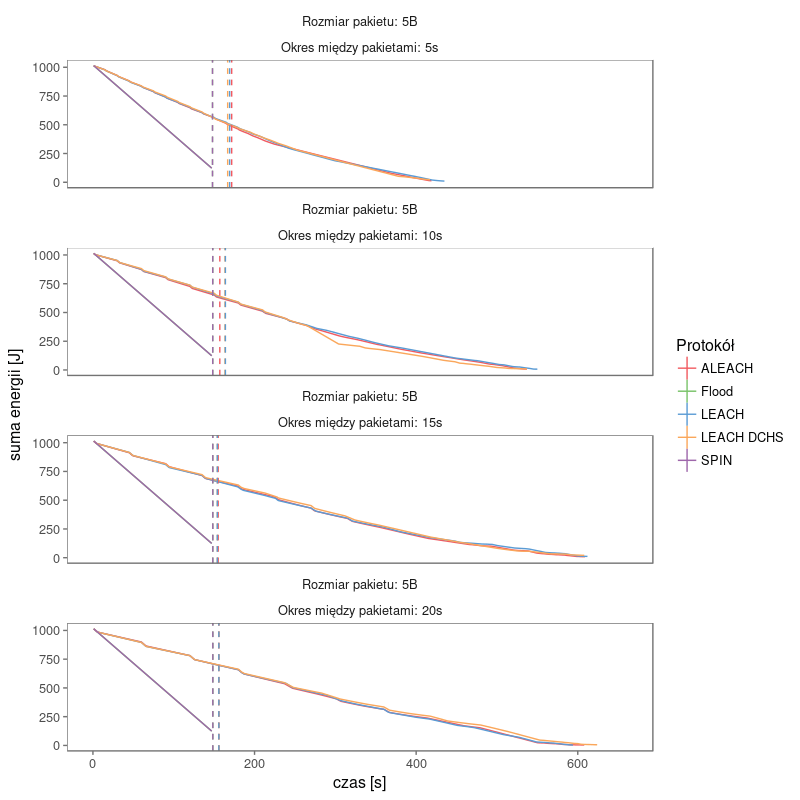
\includegraphics[scale=0.6]{\ImgPath/charts/stored_energy_normal_200sensors_row1.png}
	\end{center}
	\caption{Energia sieci - liczba czujników: 200, rozmiar pakietu danych: 5B, rozkład normalny}
\end{figure}

Długości wykresów dla pakietów o~rozmiarze 50B są podobne do tych o~rozmiarze 5B. Można w~nich zauważyć tożsame tendencje ogólne. Warto zwrócić uwagę na zmiany, jakie w~poszczególnych wykresach prezentuje protokół LEACH DCHS. Dla okresów między pakietami wynoszącym 5s, w~drugiej połowie swojej długości szybciej od innych protokołów zaczął wytracać energię, natomiast dla okresów między pakietami o~długości 20s najwolniej wytracał energię.

\begin{figure}[H]
	\begin{center}
		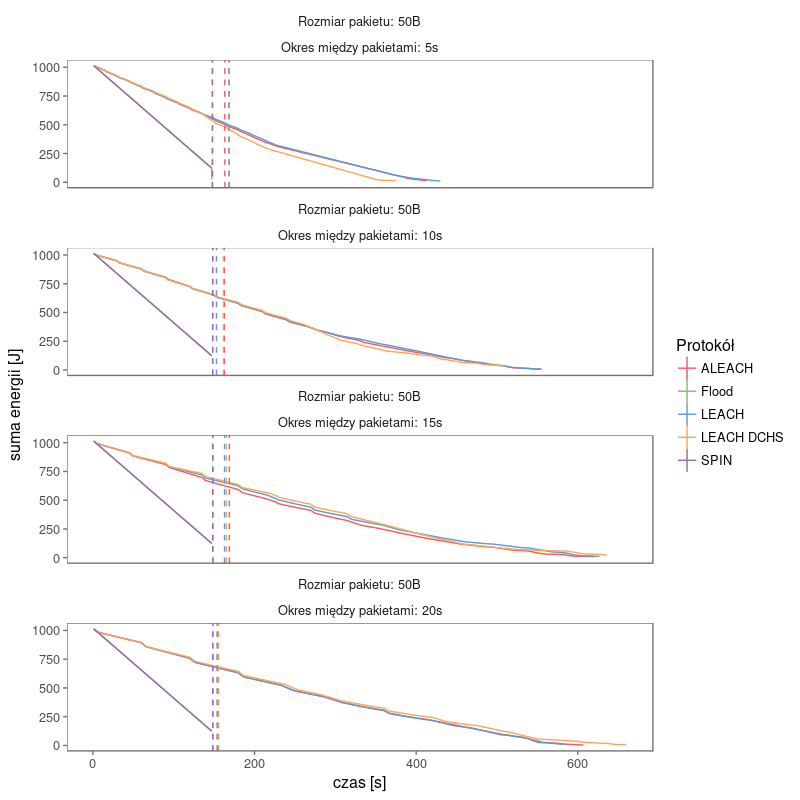
\includegraphics[scale=0.6]{\ImgPath/charts/stored_energy_normal_200sensors_row2.png}
	\end{center}
	\caption{Energia sieci - liczba czujników: 200, rozmiar pakietu danych: 50B, rozkład normalny}
\end{figure}

W opisanych poprzednio wykresach można zaobserwować zmianę w~tych, dla których rozmiar pakietów danych wynosił 500B. Różnica między protokołem SPIN, a~pozostałymi protokołami jest mniejsza, jednak zwiększa się ona wraz ze wzrostem długości odstępu pomiędzy kolejnymi pakietami z~danymi. Ogólną tendencją, która wystąpiła w~wykresach dla pakietów danych o~rozmiarze 500B jest szybsze wytracania energii. Jest to szczególnie widoczne, gdy przerwa między pakietami jest krótsza.

\begin{figure}[H]
	\begin{center}
		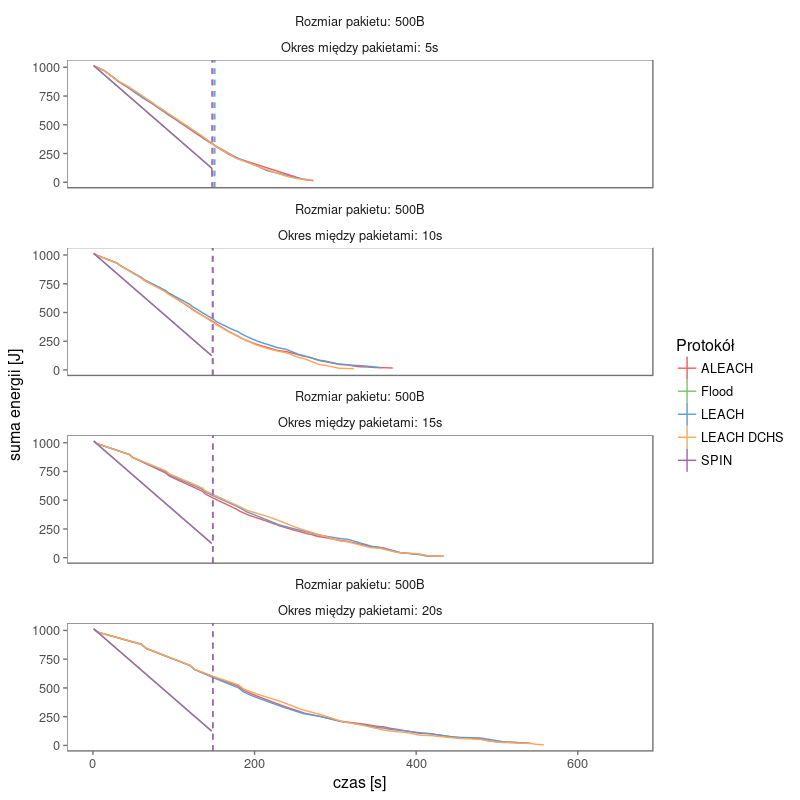
\includegraphics[scale=0.6]{\ImgPath/charts/stored_energy_normal_200sensors_row3.png}
	\end{center}
	\caption{Energia sieci - liczba czujników: 200, rozmiar pakietu danych: 500B, rozkład normalny}
\end{figure}

Najbardziej odbiegające od pierwszych wykresów są te, które przedstawiają pakiety o~rozmiarze 5000B. Tu protokoły ALEACH, LEACH i~LEACH DCHS bardzo zbliżyły się do sumy energii sieci używającej protokołu SPIN. Wykresy tej grupy są też najkrótsze spośród wszystkich.

\begin{figure}[H]
	\begin{center}
		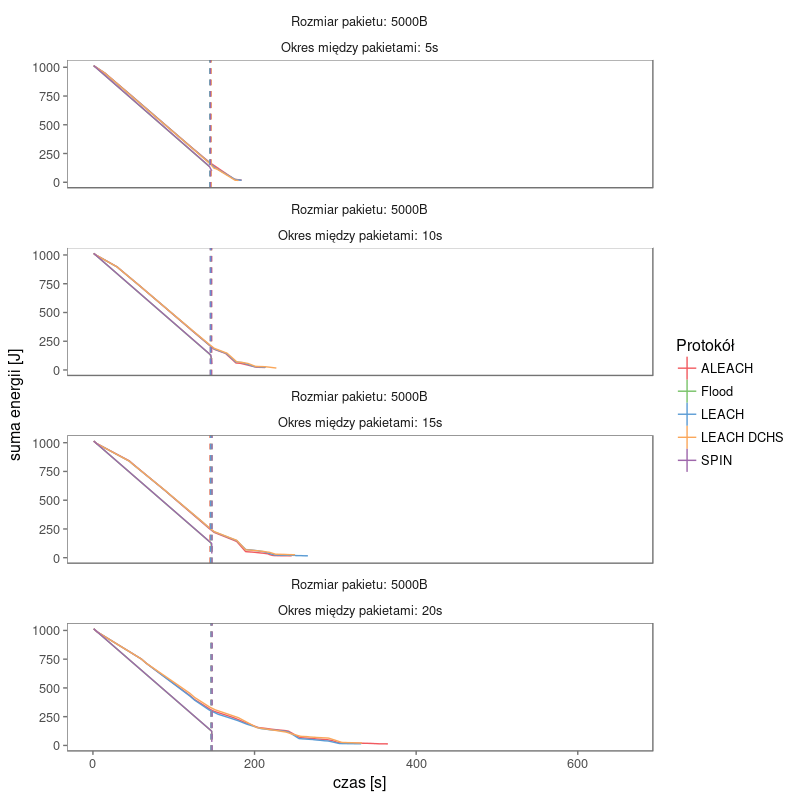
\includegraphics[scale=0.6]{\ImgPath/charts/stored_energy_normal_200sensors_row4.png}
	\end{center}
	\caption{Energia sieci - liczba czujników: 200, rozmiar pakietu danych: 5000B, rozkład normalny}
\end{figure}

Na wykresach zaprezentowano liczbę aktywnych czujników w~zależności od rodzaju protokołu, rozmiaru pakietu i~okresów między pakietami. Sieć składała się z~dwudziestu węzłów, które rozmieszczone zostały zgodnie z~rozkładem jednorodnym.
Ogólnym trendem, który można zaobserwować w~całej macierzy jest stopniowe skracanie się długości wykresu wraz ze wzrostem rozmiaru pakietu z~danymi. Można również zauważyć, że wykresy, w~których odstępy pomiędzy pakietami danych są dłuższe mają łagodniejszy i~co za tym idzie dłuższy przebieg.
Dla rozmiaru pakietu równego 5B można dostrzec najdłuższy przebieg protokołu ALEACH. Jest to najbardziej widoczne w~wykresach dla odstępów między pakietami równymi 15s i~20s. Pozostałe protokoły miały podobny przebieg. Najmniejsze różnice między ALEACH, a~pozostałymi protokołami widoczne są na wykresie z~czasem między pakietami równym 5s. Dla tej grupy wykresów najbardziej widoczną tendencją jest wydłużający się przebieg wykresów wraz ze wzrostem przerwy między pakietami. 

\begin{figure}[H]
	\begin{center}
		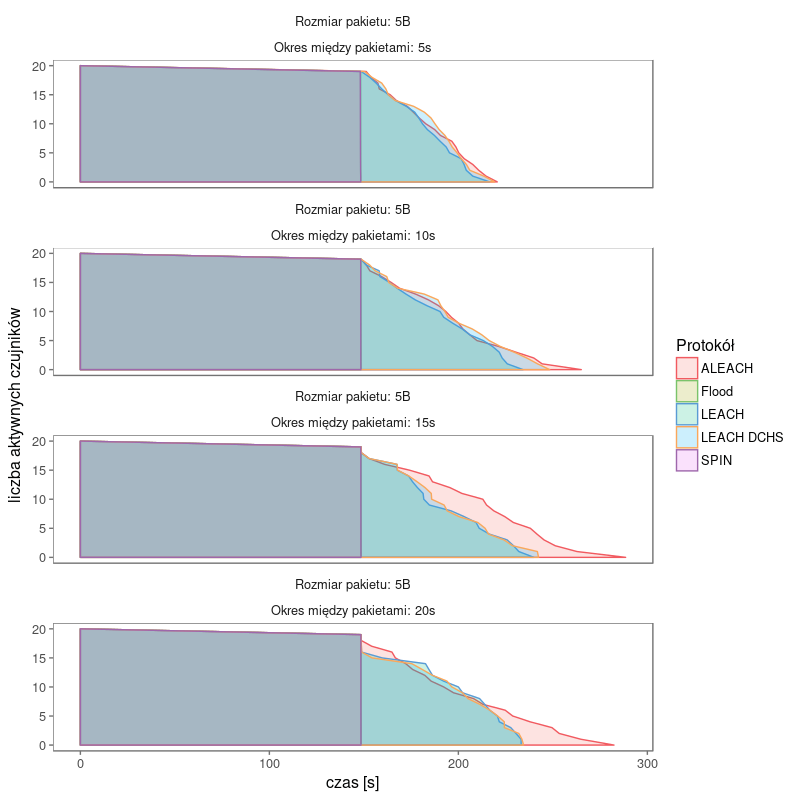
\includegraphics[scale=0.6]{\ImgPath/charts/alive_nodes_uniform_20sensors_row1.png}
	\end{center}
	\caption{Aktywne węzły - liczba czujników: 20, rozmiar pakietu danych: 5B, rozkład jednorodny}
\end{figure}

Na wykresach dla rozmiaru pakietu danych 50B można zaobserwować podobny przebieg, jak dla tych wizualizujących eksperymenty ,w których ta wartość wynosiła 5B, jednak widać kilka różnic między nimi. Linie poszczególnych protokołów nie nakładają się na siebie już w~tak znaczący sposób, widać różnice pomiędzy nimi. Najlepsze wyniki, a~więc najdłuższe działanie miał protokół ALEACH, który niezależnie od okresów między pakietami wykazał najłagodniejszy przebieg. Sytuacją, na którą warto zwrócić uwagę jest ta, która ma miejsce na wykresie dla czasu między pakietami równemu 15s. Tu zdecydowanie najkrótszy przebieg miał protokół LEACH.

\begin{figure}[H]
	\begin{center}
		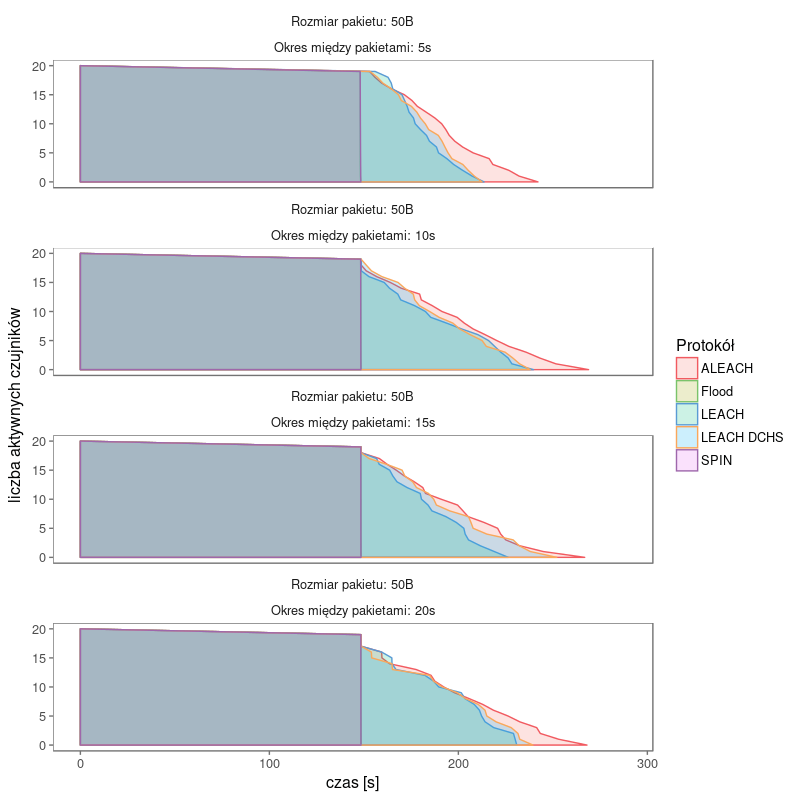
\includegraphics[scale=0.6]{\ImgPath/charts/alive_nodes_uniform_20sensors_row2.png}
	\end{center}
	\caption{Aktywne węzły - liczba czujników: 20, rozmiar pakietu danych: 50B, rozkład jednorodny}
\end{figure}

 Podany wcześniej opis wykresów dla rozmiaru 50B mógłby być jednocześnie opisem tych dla rozmiaru 500B. Warto zwrócić uwagę na podobny przebieg protokołu LEACH na wykresie z~okresami między pakietami równymi 15s. Był on krótszy od pozostałych protokołów. Różnica między protokołem ALEACH a~pozostałymi protokołami była tym większa, im dłuższe były okresy między pakietami.

\begin{figure}[H]
	\begin{center}
		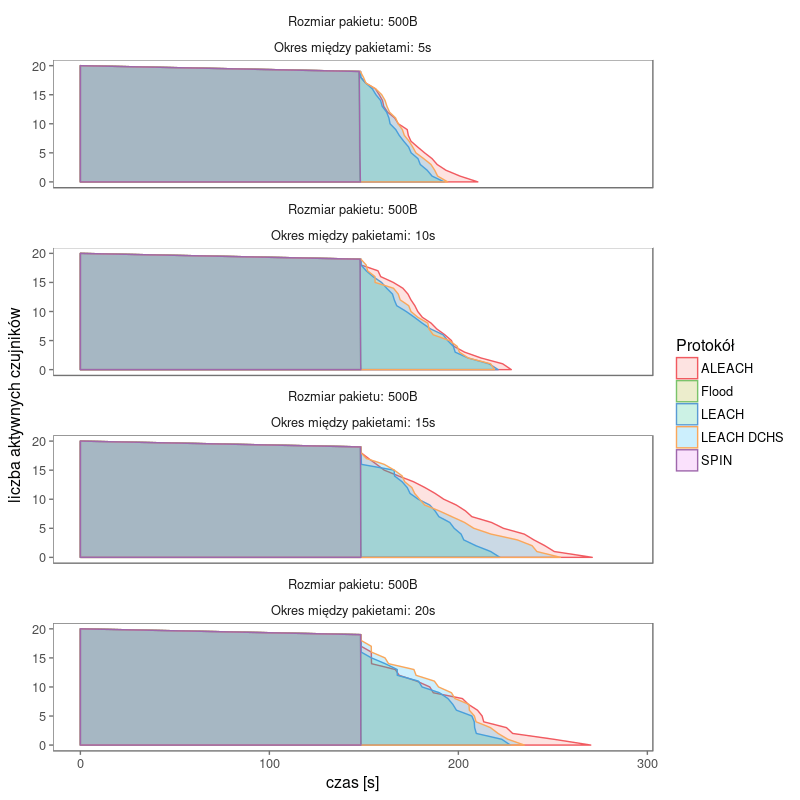
\includegraphics[scale=0.6]{\ImgPath/charts/alive_nodes_uniform_20sensors_row3.png}
	\end{center}
	\caption{Aktywne węzły - liczba czujników: 20, rozmiar pakietu danych: 500B, rozkład jednorodny}
\end{figure} 
  
Liczba aktywnych czujników malała najszybciej w~wykresach o~rozmiarze 5000B. Tu różnica między ALEACH, a~pozostałymi protokołami była widoczna tylko na wykresie o~okresie między pakietami równym 20s. W~pozostałych protokoły miały podobny przebieg. 

\begin{figure}[H]
	\begin{center}
		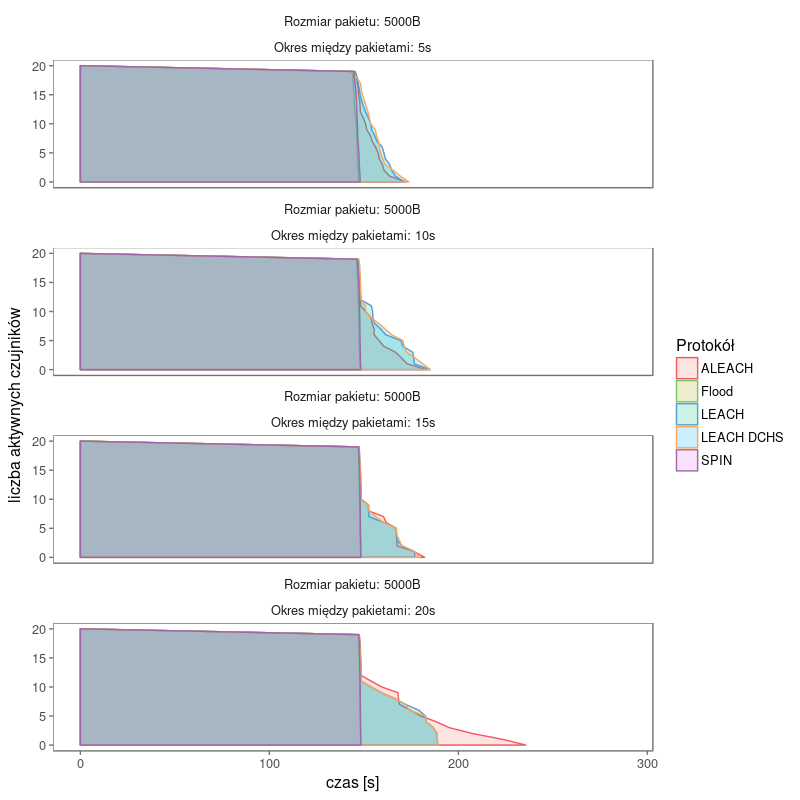
\includegraphics[scale=0.6]{\ImgPath/charts/alive_nodes_uniform_20sensors_row4.png}
	\end{center}
	\caption{Aktywne węzły - liczba czujników: 20, rozmiar pakietu danych: 5000B, rozkład jednorodny}
\end{figure}


Na poniższych wykresach przedstawiono zależności między sumą energii wyrażonej w~dżulach a~czasem, rozmiarem pakietu oraz okresami między pakietami. Sieć składała się z~dwudziestu węzłów, które rozmieszczone zostały zgodnie z~rozkładem jednorodnym.
Na przedstawionych wykresach można zauważyć kilka wspólnych trendów. Pierwszym z~nich jest inny od pozostałych przebieg protokołu SPIN, w~przypadku którego energia jest szybciej wytracana. Warto zwrócić uwagę też na protokół ALEACH, którego wykres najczęściej był najdłuższy. Zależność ta jest najbardziej widoczna na wykresach o~okresie między pakietami równym 15s i~20s. Ogólny przebieg wykresów protokołów (z wyjątkiem protokołu SPIN) był zbliżony. Można na wykresach zaobserwować trend wolniejszego wytracania energii wraz ze wzrostem okresów między pakietami.

Na wykresach dla rozmiaru pakietu 5B można zaobserwować największą różnicę pomiędzy protokołem SPIN a~pozostałymi protokołami. Na uwagę zasługuje również zależność dla protokołu ALEACH, dla którego sieć tym wolniej wytraca energię im dłuższy jest okres między pakietami. Najbardziej zbliżony przebieg protokołów (z wyjątkiem protokołu SPIN) można zaobserwować na wykresie dla okresów między pakietami równemu 5s. Niewielkie różnice pojawiają się wraz ze wzrostem odstępu czasu pomiędzy pakietami danych.

\begin{figure}[H]
	\begin{center}
		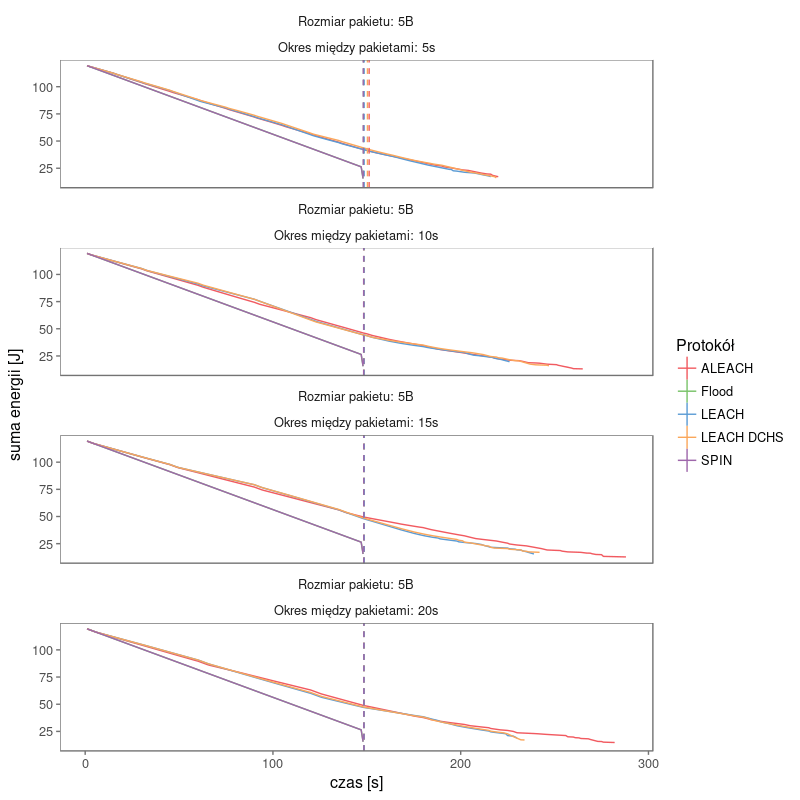
\includegraphics[scale=0.6]{\ImgPath/charts/stored_energy_uniform_20sensors_row1.png}
	\end{center}
	\caption{Energia sieci - liczba czujników: 20, rozmiar pakietu danych: 5B, rozkład jednorodny}
\end{figure}
 
Wykresy o~rozmiarach 50B i~500B mają podobny przebieg. Można tu zauważyć podobne trendy jak na wykresach o~rozmiarze 5B. Warto zwrócić uwagę, że różnica między protokołem SPIN na wykresach o~rozmiarze 50B jest relatywnie podobna, natomiast na wykresach o~rozmiarze 500B rośnie wraz z~wydłużeniem się odstępu między pakietami. Na wykresach o~odstępach między pakietami danych równemu 15s protokół LEACH nieco szybciej wytraca energię w~okolicach 180 sekundy działania sieci.

\begin{figure}[H]
	\begin{center}
		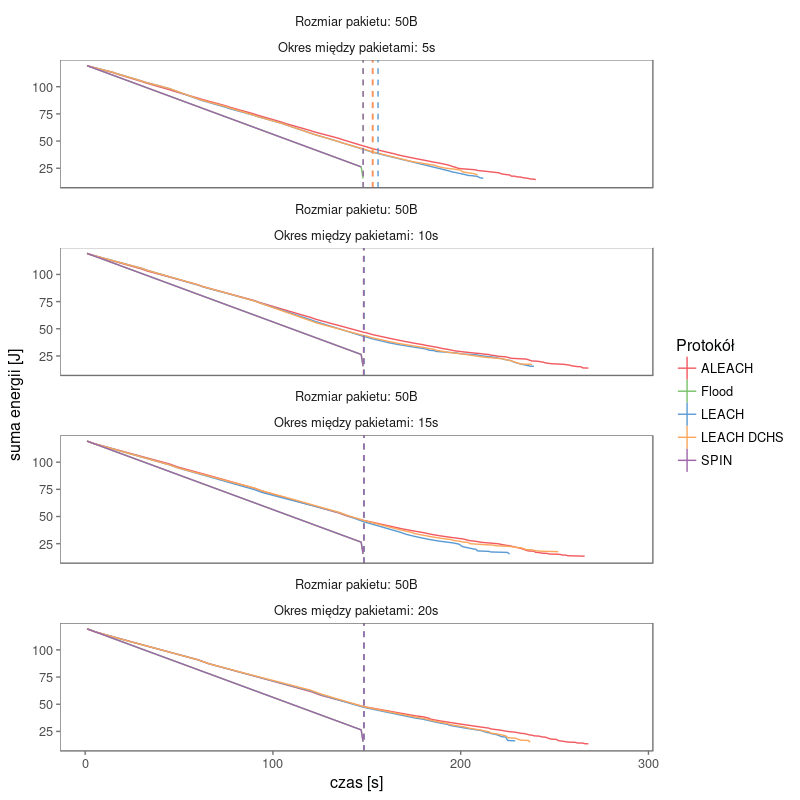
\includegraphics[scale=0.6]{\ImgPath/charts/stored_energy_uniform_20sensors_row2.png}
	\end{center}
	\caption{Energia sieci - liczba czujników: 20, rozmiar pakietu danych: 50B, rozkład jednorodny}
\end{figure}

\begin{figure}[H]
	\begin{center}
		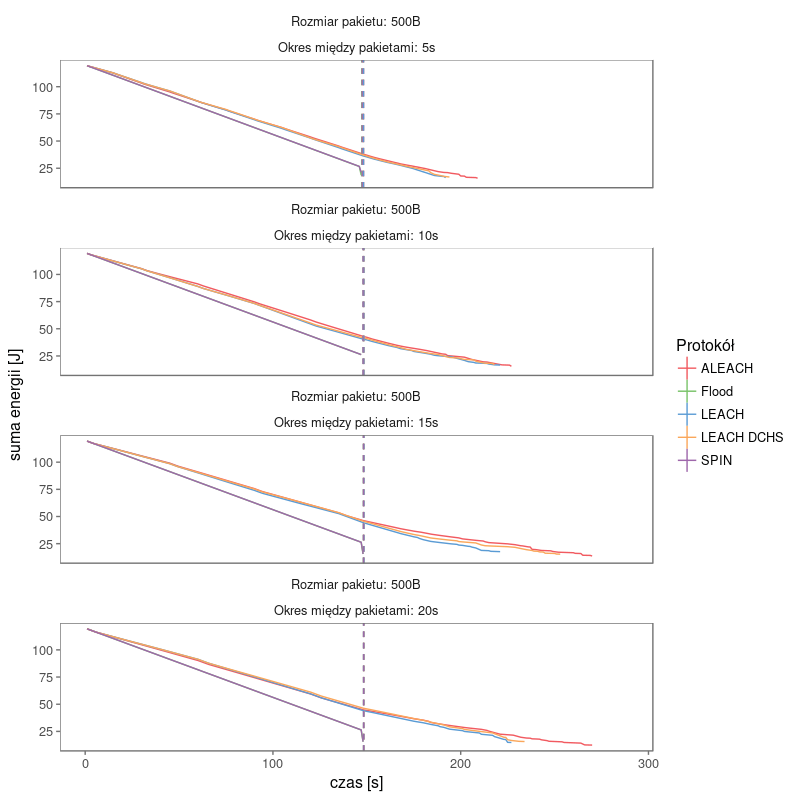
\includegraphics[scale=0.6]{\ImgPath/charts/stored_energy_uniform_20sensors_row3.png}
	\end{center}
	\caption{Energia sieci - liczba czujników: 20, rozmiar pakietu danych: 500B, rozkład jednorodny}
\end{figure}
 
Wykresy pakietów o~rozmiarze 5000B różnią się od pozostałych. Tu różnica między protokołem SPIN, a~pozostałymi protokołami jest najmniejsza, a~na wykresach o~czasie między pakietami równym 5s i~10s jest niezauważalna. Warto zwrócić uwagę na przebieg protokołu ALEACH dla odstępów równych 20s. Tu jest on zdecydowanie dłuższy od pozostałych. 

\begin{figure}[H]
	\begin{center}
		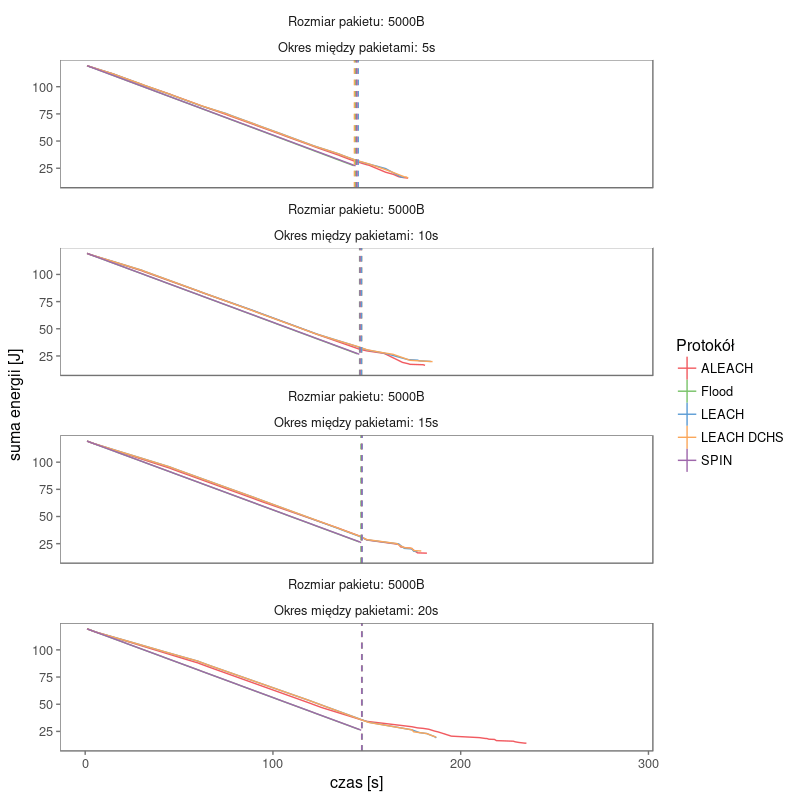
\includegraphics[scale=0.6]{\ImgPath/charts/stored_energy_uniform_20sensors_row4.png}
	\end{center}
	\caption{Energia sieci - liczba czujników: 20, rozmiar pakietu danych: 5000B, rozkład jednorodny}
\end{figure}

Na poniższych wykresach przedstawiono zależność pomiędzy liczbą aktywnych czujników a~czasem, rozmiarem pakietu i~okresami między pakietami dla różnych protokołów. Sieć składała się z~dwustu węzłów, które rozmieszczone zostały zgodnie z~rozkładem jednorodnym.
Wykresy dla rozmiaru pakietu danych 5B są dość zróżnicowane. W~przypadku okresów między pakietami równym 5s i~15s warto zwrócić uwagę na najszybsze zmniejszanie liczby aktywnych czujników przy zastosowaniu protokołu LEACH DCHS. Wykresem, który najwolniej opadał był w~tych przypadkach ten, który ilustruje protokół LEACH. Podobne zróżnicowanie można zaobserwować przy wykresie dla okresów między pakietami równych 10s, jednak z~tą różnicą, że punkt końcowy jest zbliżony dla wszystkich protokołów. Odmiennym wykresem od pozostałych jest ten dla odstępów między pakietami równych 20s. Tu liczba aktywnych czujników jest zbliżona we wszystkich protokołach.

\begin{figure}[H]
	\begin{center}
		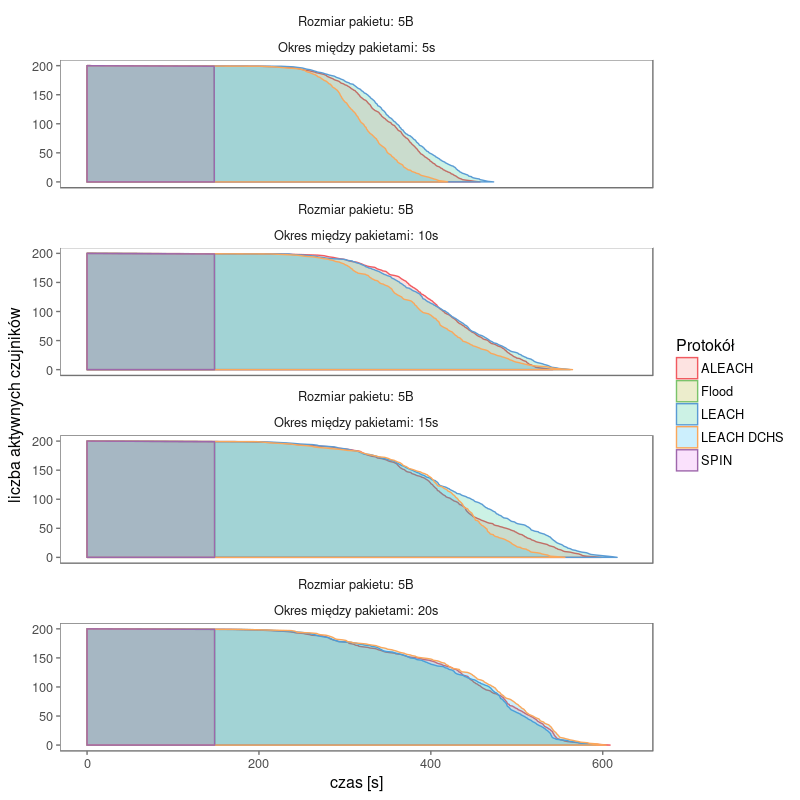
\includegraphics[scale=0.6]{\ImgPath/charts/alive_nodes_uniform_200sensors_row1.png}
	\end{center}
	\caption{Aktywne węzły - liczba czujników: 200, rozmiar pakietu danych: 5B, rozkład jednorodny}
\end{figure}

Różnice w~przebiegu wykresów ilustrujących ilość aktywnych czujników dla różnych protokołów można zauważyć również w~przypadku pakietów o~rozmiarze 50B. Warto zwrócić uwagę na protokół LEACH DCHS, który dla okresów między pakietami 5s, 10s, 15s przyjmuje wartości niższe, a~w~przypadku okresów równych 20s momentami wyższe od innych protokołów.  Z~wyjątkiem protokołu LEACH DCHS wszystkie protokoły miały zbliżony przebieg. Dla okresów między pakietami równych 10s i~15s protokołem, po którego zastosowaniu czujniki pozostały najdłużej aktywne był ALEACH.

\begin{figure}[H]
	\begin{center}
		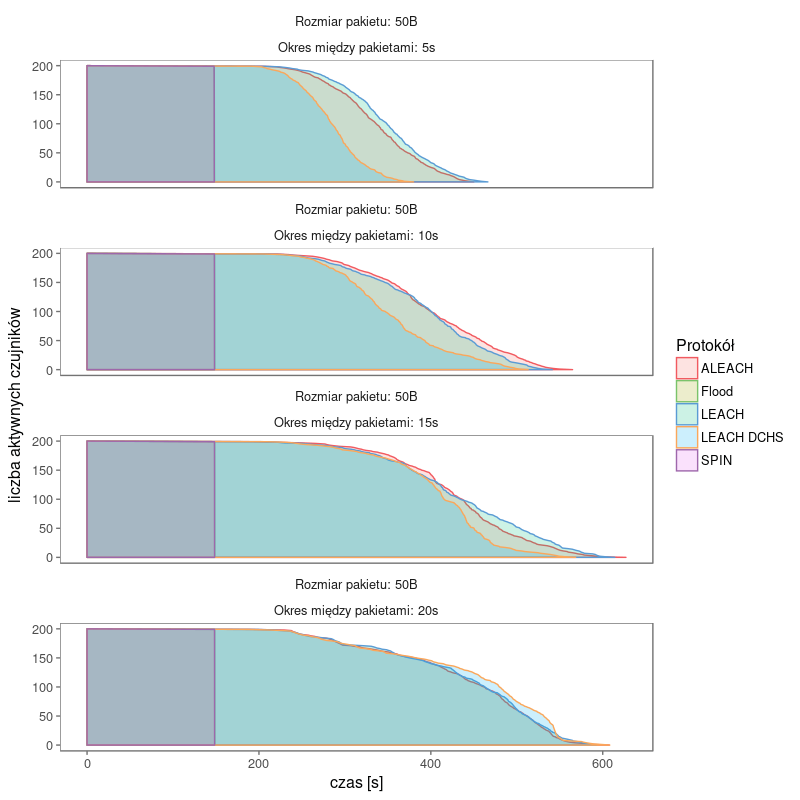
\includegraphics[scale=0.6]{\ImgPath/charts/alive_nodes_uniform_200sensors_row2.png}
	\end{center}
	\caption{Aktywne węzły - liczba czujników: 200, rozmiar pakietu danych: 50B, rozkład jednorodny}
\end{figure}

Wykresy pakietów o~rozmiarze 500B są znacznie krótsze od opisywanych wcześniej, a~więc liczba aktywnych czujników zmniejsza się szybciej. Warto zwrócić uwagę, że różnica między protokołami nie jest już zauważalna. Wykresy są dłuższe w~miarę wydłużania się okresów między pakietami.

\begin{figure}[H]
	\begin{center}
		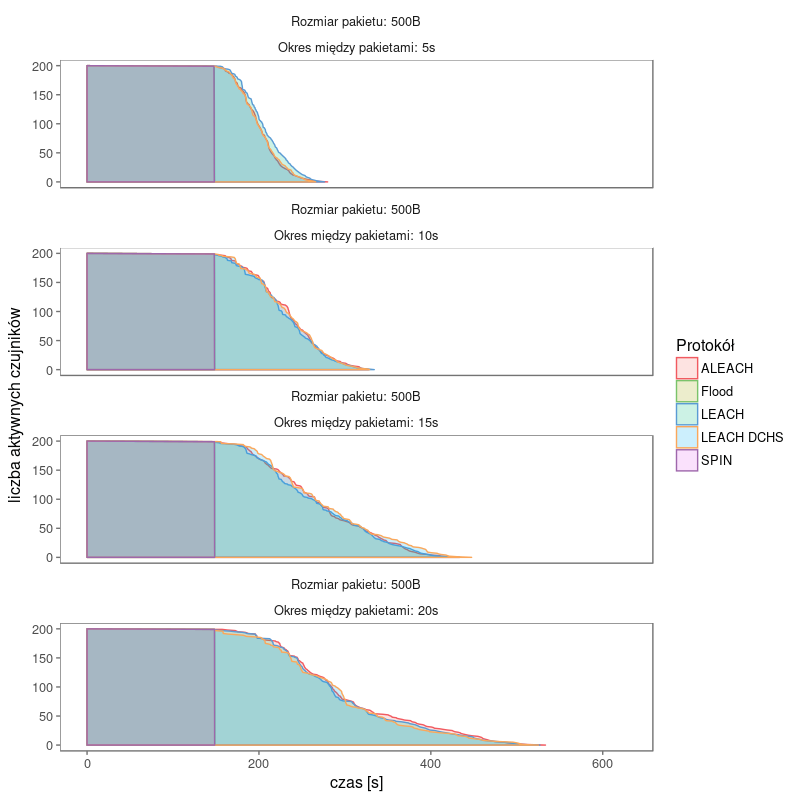
\includegraphics[scale=0.6]{\ImgPath/charts/alive_nodes_uniform_200sensors_row3.png}
	\end{center}
	\caption{Aktywne węzły - liczba czujników: 200, rozmiar pakietu danych: 500B, rozkład jednorodny}
\end{figure}

Na rysunku \ref{fig:aliveNodesUniform200sensorsRow4} znajdują się wykresy dla pakietów danych o~rozmiarze 5000B. Wykresy te są najkrótsze w~całej macierzy, a~ten dla okresów między pakietami równych 5s jest krótszy niż 200 sekund. Pierwsze trzy wykresy posiadają zbliżony przebieg protokołów. Jedynie na wykresie dla czasu między kolejnymi pakietami z~danymi równemu 20s można zaobserwować różnice między poszczególnymi protokołami, jednak zakończenie działania ostatniego czujnika jest zbliżone we wszystkich z~nich.

\begin{figure}[H]
	\begin{center}
		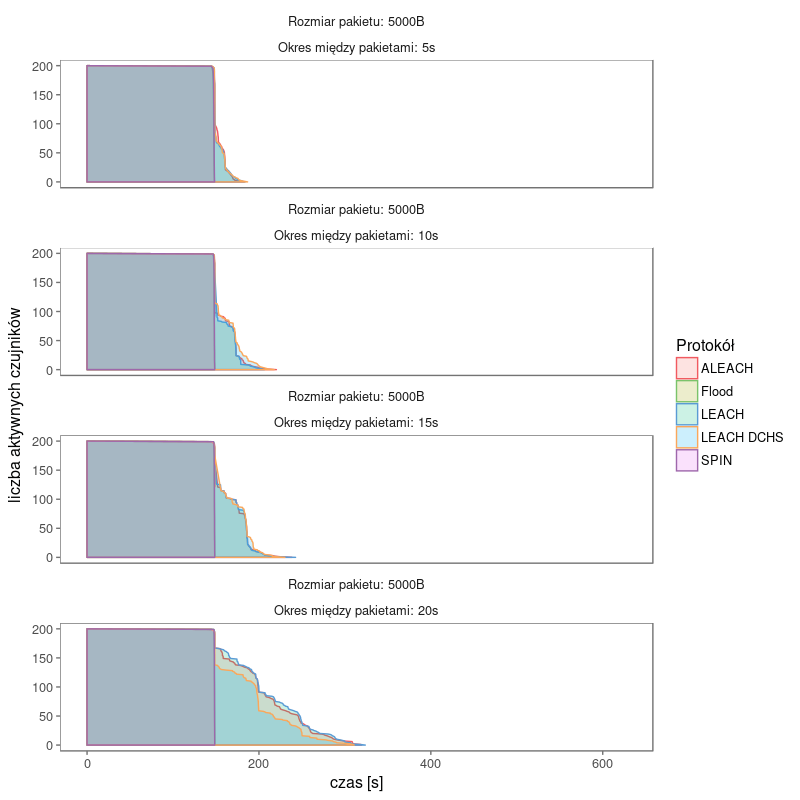
\includegraphics[scale=0.6]{\ImgPath/charts/alive_nodes_uniform_200sensors_row4.png}
	\end{center}
	\caption{Aktywne węzły - liczba czujników: 200, rozmiar pakietu danych: 5000B, rozkład jednorodny}
	\label{fig:aliveNodesUniform200sensorsRow4}
\end{figure}

Na wykresach zobrazowano zależność pomiędzy sumą energii wyrażoną w~dżulach a~rozmiarem pakietu, okresami między pakietami dla różnych protokołów. Sieć składała się z~dwustu węzłów, które rozmieszczone zostały zgodnie z~rozkładem jednorodnym.

Wykresy dla pakietów o~rozmiarze 5B charakteryzują się najwolniejszym spadkiem sumy energii sieci. Zależność ta wzrasta wraz z~wydłużaniem się okresów między pakietami. Protokołem najszybciej wytracającym energię był SPIN. Wykresy obrazujące sumę energii przy zastosowaniu pozostałych protokołów posiadają podobny przebieg. Niewielkie różnice między protokołami można zaobserwować w~przypadku okresów równych 15s. Tu najwolniej suma energii malała przy zastosowaniu protokołu LEACH.

\begin{figure}[H]
	\begin{center}
		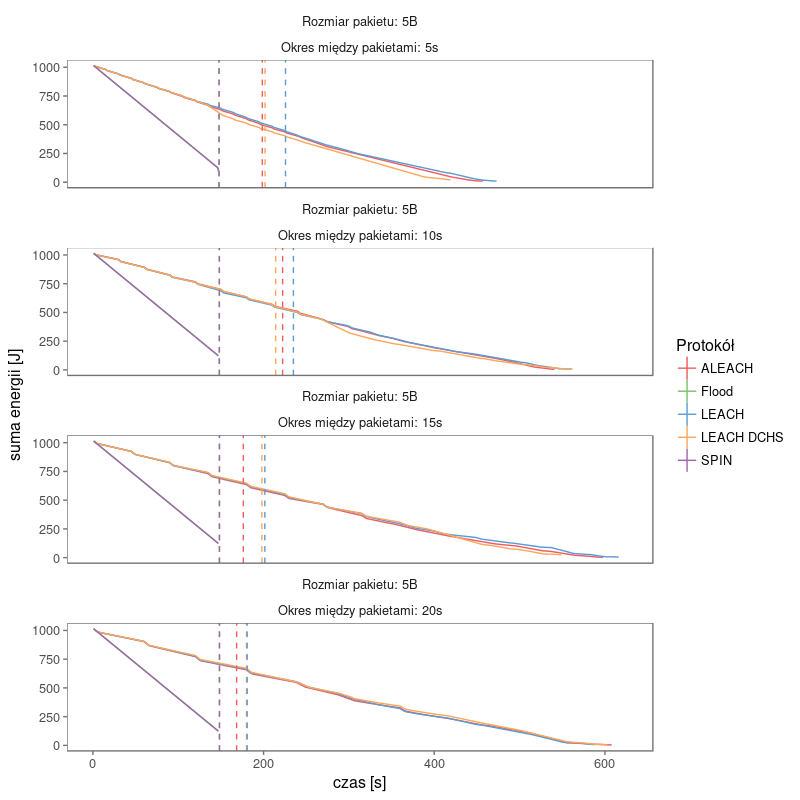
\includegraphics[scale=0.6]{\ImgPath/charts/stored_energy_uniform_200sensors_row1.png}
	\end{center}
	\caption{Energia sieci - liczba czujników: 200, rozmiar pakietu danych: 5B, rozkład jednorodny}
\end{figure}

Przebieg podobnej długości do wykresów w~których rozmiar pakietu danych wynosił 5B prezentują te o~wielkości 50B. W~ich przypadku można dostrzec dużą różnicę pomiędzy SPIN a~pozostałymi protokołami.  Warto zwrócić uwagę na przebieg protokołu LEACH DCHS, w~przypadku którego szybciej od pozostałych jest zużywana energia sieci. Różnica ta zmniejsza się wraz ze wzrostem okresów między pakietami. 

\begin{figure}[H]
	\begin{center}
		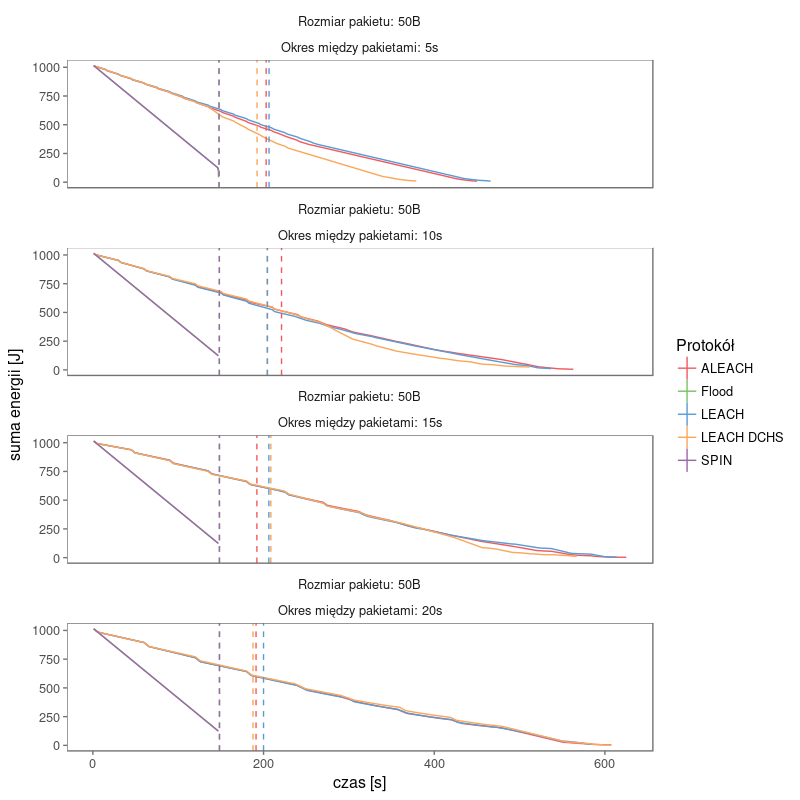
\includegraphics[scale=0.6]{\ImgPath/charts/stored_energy_uniform_200sensors_row2.png}
	\end{center}
	\caption{Energia sieci - liczba czujników: 200, rozmiar pakietu danych: 50B, rozkład jednorodny}
\end{figure}

Wykresy dla pakietów danych o~rozmiarze 500B obrazują szybsze zużycie energii sieci od poprzednich.  Można zaobserwować zmniejszenie się różnicy między przebiegiem SPIN a~pozostałymi protokołami. Widoczna jest również tendencja tym wolniejszego spadku sumy energii im dłuższy jest okres między pakietami. Protokoły z~wyjątkiem SPIN  posiadały podobny przebieg.

\begin{figure}[H]
	\begin{center}
		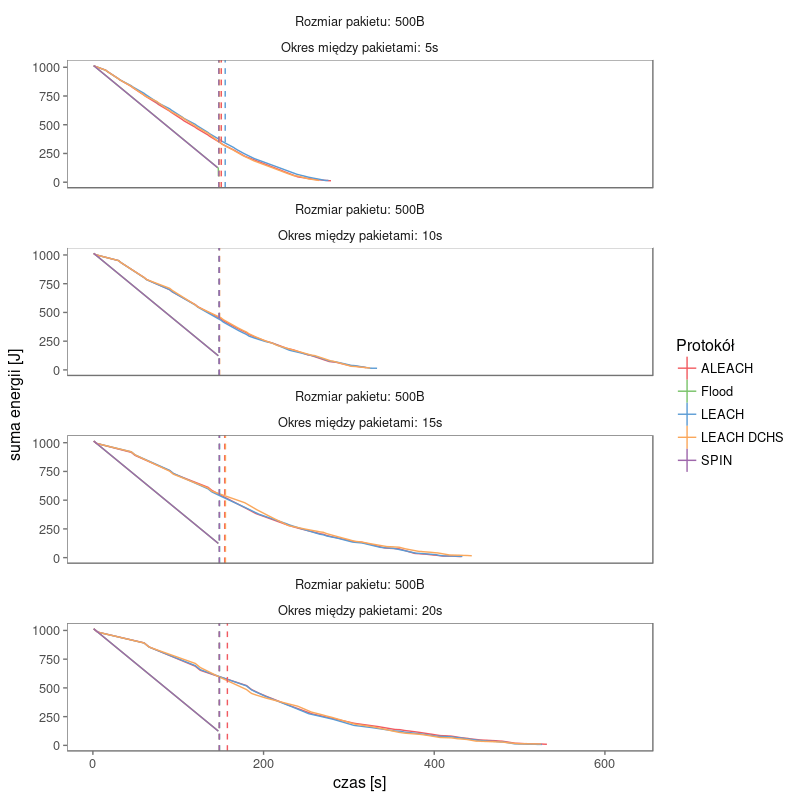
\includegraphics[scale=0.6]{\ImgPath/charts/stored_energy_uniform_200sensors_row3.png}
	\end{center}
	\caption{Energia sieci - liczba czujników: 200, rozmiar pakietu danych: 500B, rozkład jednorodny}
\end{figure}

Wykresami prezentującymi najszybsze zużycie energii są te dla rozmiaru pakietu danych równemu 5000B. Najkrótszym wykresem jest ten dla okresów między pakietami o~długości 5s, który jako jedyny w~całej macierzy przedstawia czas działania sieci trwający mniej niż 200s. Warto zwrócić uwagę, że wszystkie protokoły, także SPIN, mają tu podobny przebieg. Różnica między SPIN a~pozostałymi protokołami jest tym większa im dłuższy jest okres między pakietami.


\begin{figure}[H]
	\begin{center}
		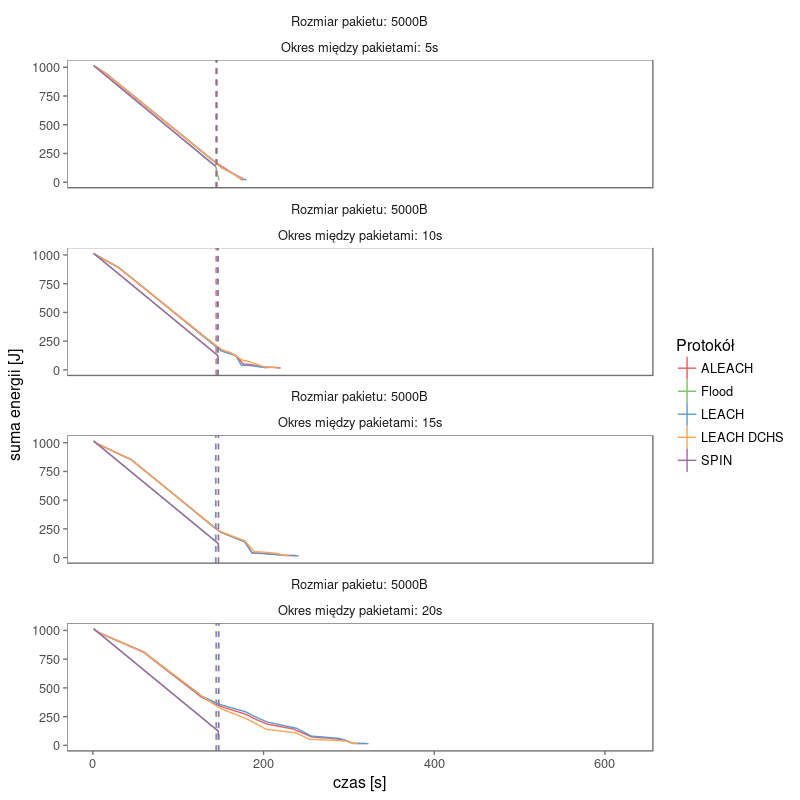
\includegraphics[scale=0.6]{\ImgPath/charts/stored_energy_uniform_200sensors_row4.png}
	\end{center}
	\caption{Energia sieci - liczba czujników: 200, rozmiar pakietu danych: 5000B, rozkład jednorodny}
\end{figure}
